\section{The Fabry-Perot Interferometer}
Optical resonators were utilized as helpful gadgets as early as 1899 when Fabry and Perot depicted the utilization of a parallel-plate resonator as a multipass interferometer. Part of the incident light on this Fabry– Perot resonator is transmitted and another part is reflected, with power divisions that rely upon numerous factors. A simple illustration of the basic Fabry-Perot is shown in Figure 2.1, here $r_{1} t_{1}$ are the reflectivity constant and transmitivity constant of the mirror 1 respectively and $r_{2} t_{2}$ are the reflectivity and transmitivity constants of the mirror two respectively. Also, $E_{i}$ is the incident Electromagnetic energy, $E_{t}$ is the transmitted energy and $E_{r}$ is the reflected energy. This is an asymmetric Fabry-Perot resonator:

\begin{figure}[h]
\centering
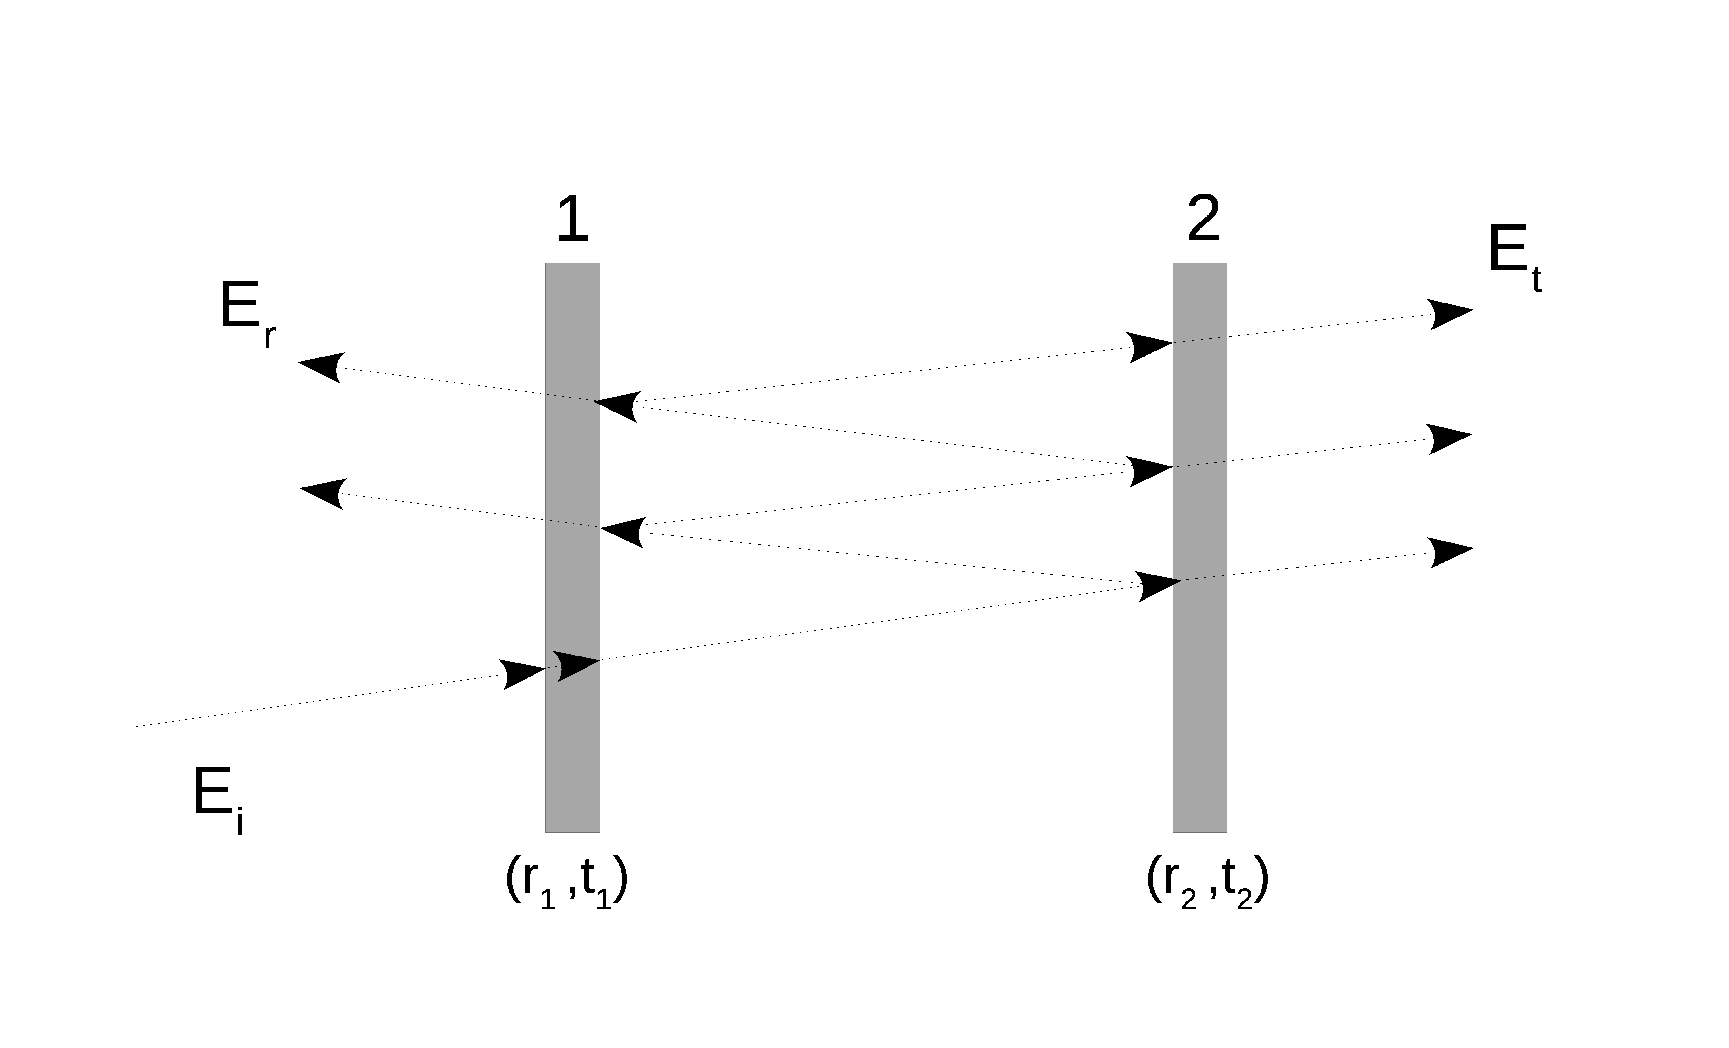
\includegraphics[width=0.60\textwidth]{Fabry_Perot_resonator.eps}
\caption{Illustrated energy diagram of a simple Fabry-Perot resonator}
\end{figure}



\newpage

\subsection{Theory of Fabry-Perot Interferometer}
If the incident energy is in the form of white coherent light then at that point the transmission and reflection coefficients depend just on the mirror reflectivities. The total reflected power comprises of the power reflected from the principal mirror in addition to all the different reflections between the mirrors that add to the reflectivity in general. In summation, the equations are [1]: 
\begin{equation}
{\mathcal R} = R_{1} + T_{1}^2 R_{2} \sum_{m=1}^{\infty} (R_{1}R_{2})^{m-1} = \frac{R_{1} - 2R_{1}R_{2} + R_{2}}{1 - R_{1}R_{2}} _{\overrightarrow{R_{1} = R_{2} \equiv R}} \frac{2R}{1+R}
\end{equation}

Similarly, the transmitted energy in summation is:
\begin{equation}
{\mathcal T} = T_{1} T_{2} \sum_{m=1}^{\infty} (R_{1}R_{2})^{m-1} = \frac{T_{1} T_{2}}{1 - R_{1}R_{2}} _{\; \overrightarrow{R_{1} = R_{2} \equiv R}} \; \frac{T^{2}}{1-R^{2}} = \frac{1-R}{1+R}
\end{equation}

Assuming, be that as it may, the incident light comprises of a transiently lucid (monochromatic) plane wave, at that point the reflected power will be relative to the square of the modulus of every reflected field. Since the fields convey phase information as well as amplitudes of the transmission, the division of reflected and transmitted light depends not just on the mirror reflectivities but in addition on the mirror separation and excitation wavelength. The rational total of fields is amplified when every one of the fields interferes constructively (in phase) and limited when they interfere destructively (out of phase). Phase gathers with propagation separation as $\phi(z) = \beta z$ and may likewise be gained upon communication with the mirrors. The sound forms of Eqs. 2.1 and 2.2 incorporate an aggregated phase for each round-trip that can be translated as a standardized detuning $\phi = T_{R}\omega$, where $T_{R}$ is the cavity travel time, $T_{R} = n_{eff}L/c$ for the circumference L, and effective index $n_{eff}$. Presently, $\tilde{r}$ defines the complex reflectivity: 

\begin{multline}
\tilde{r} = r_{1} - t_{1}^{2}r_{2}\exp(i m \phi) \sum_{m=1}^{\infty} (r_{1}r_{2}\exp(i m \phi))^{m-1} \\ = \frac{r_{1} - r_{2}\exp(i \phi)}{1 - r_{1}r_{2}\exp(i \phi)} _{\; \overrightarrow{r_{1} = r_{2} \equiv r}} \; \frac{r(1-\exp(+i \phi))}{1-r^{2}\exp(+i \phi)}
\end{multline}

and $\tilde{t}$ represents the complex transmittivity:

\begin{multline}
\tilde{t} = -t_{1}t_{2}\exp(i m \phi/2) \sum_{m=1}^{\infty} (r_{1}r_{2}\exp(i m \phi))^{m-1} \\ = \frac{-t_{1}t_{2}\exp(i m \phi/2)}{1 - r_{1}r_{2}} _{\; \overrightarrow{r_{1} = r_{2} \equiv r}} \; \frac{-(1-r^{2})\exp(im \phi/2)}{1-r^{2}}
\end{multline}


The square modulus of these perplexing amounts gives the reflection ${\mathcal R}$ and transmission ${\mathcal T}$ coefficients (shown in Fig. 2.2). Antiresonant wavelengths are more emphatically reflected than in the ambiguous case, while resonant wavelengths are transmitted $100\%$ for adjusted reflectors ($r_{1}$ = $r_{2}$). For a fixed reflect dispersing, the transmission and reflection spectra in this manner show intermittent pinnacles and valleys. Figure 2.2 presenting the transmission and reflection spectra for a lossless, adjusted Fabry– Perot resonator. The part of reflected and transmitted power for mixed up excitation is identical to the separate spectrally averaged reflection and transmission over time of the spectrum range.

The values of reflectivity coefficients $r_{1}$, $r_{2}$ and the transmitivity coefficients $t_{1}$, $t_{2}$ are mentioned in the figure. The plot is of the intensity of the Fabry- Perot resonator versus the round trip phase of the system. This displays a $100\%$ transmission and $0\%$ reflection on the resonant frequencies. Meaning all the incident light is detected on the other side of the resonator of these specific frequencies. 

\begin{figure}[h]
\centering
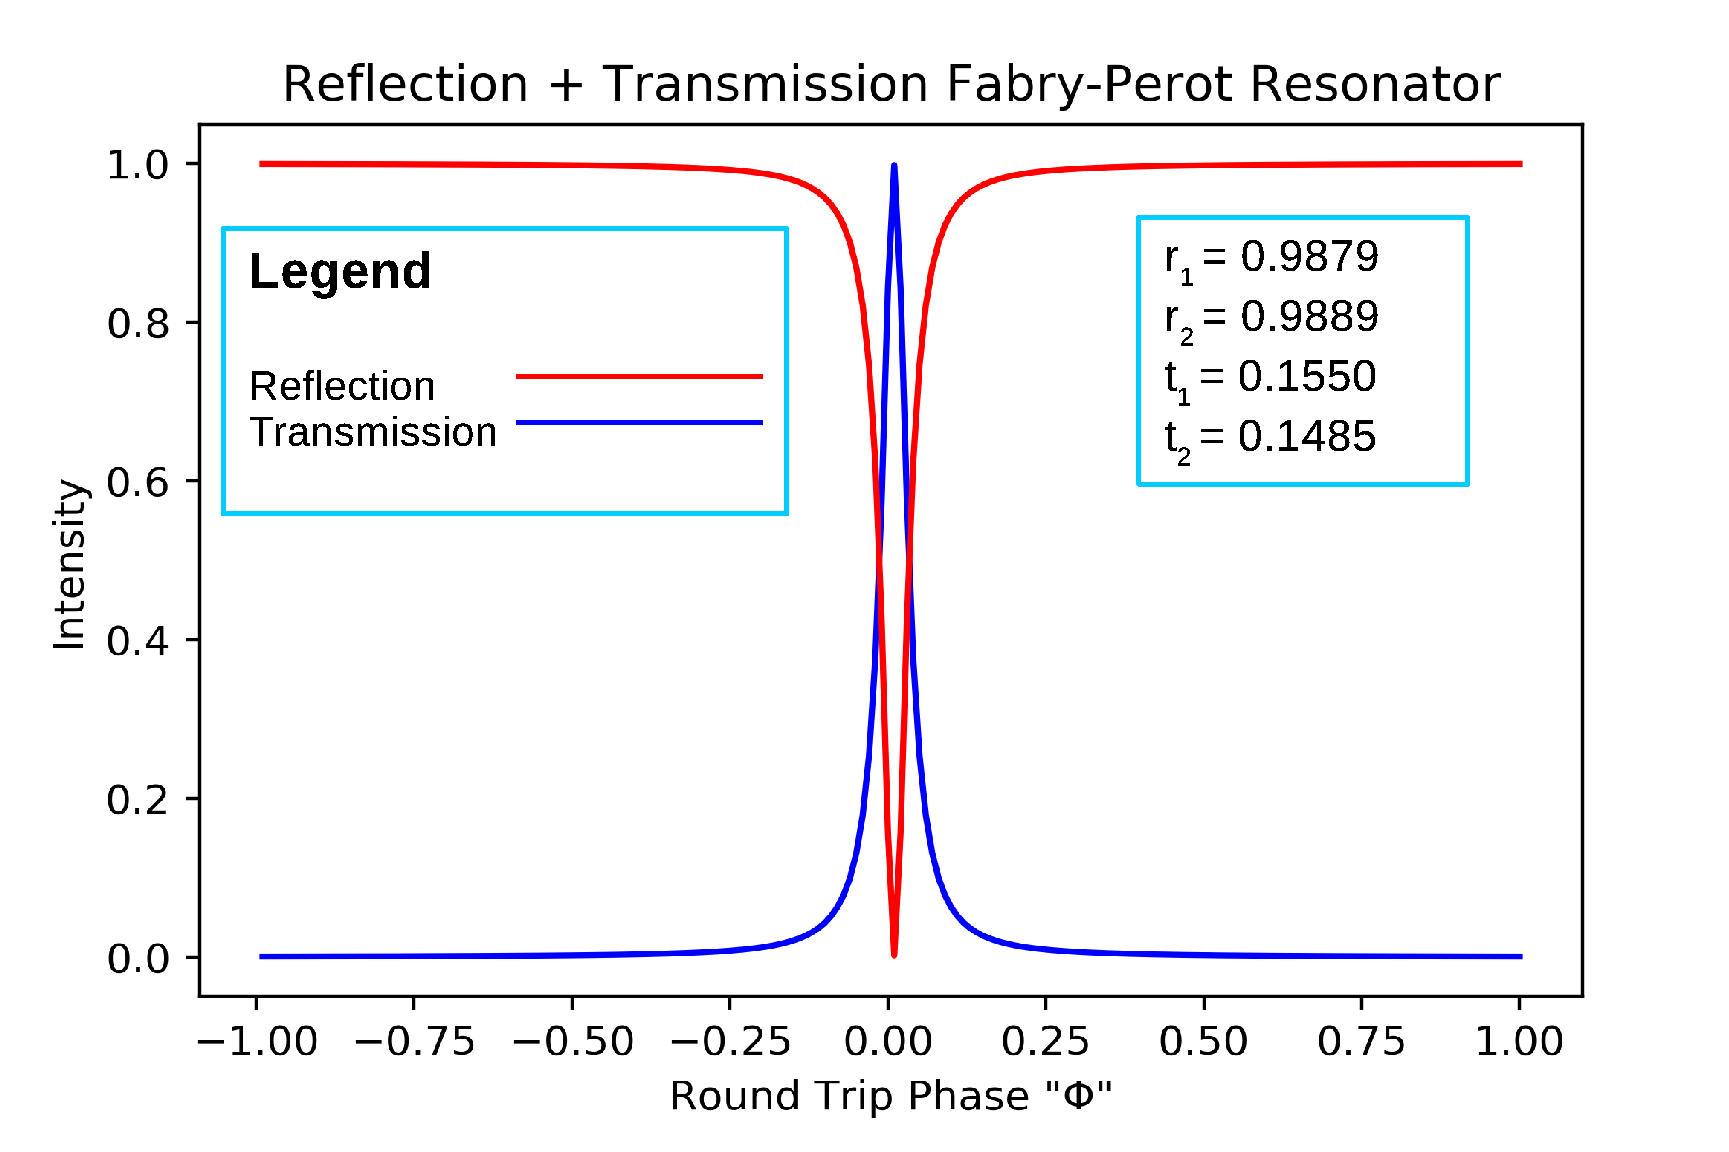
\includegraphics[width=0.85\textwidth]{R+T_FabryPerot.eps}
\caption{Transmitted and reflected field of an asymmetric Fabry-Perot resonator}
\end{figure}


\subsection{Effective Phase}
Now let us look at the phase details of the transmission and the reflection spectra of the asymmetric Fabry-Perot resonator. The phase gives us a lot of details about the traveling light inside the resonator and gives other details about dispersion, group delay, and group index. Fig. 2.3 shows phases of both transmission and reflection of an asymmetric Fabry-Perot resonator.

\begin{figure}[h]
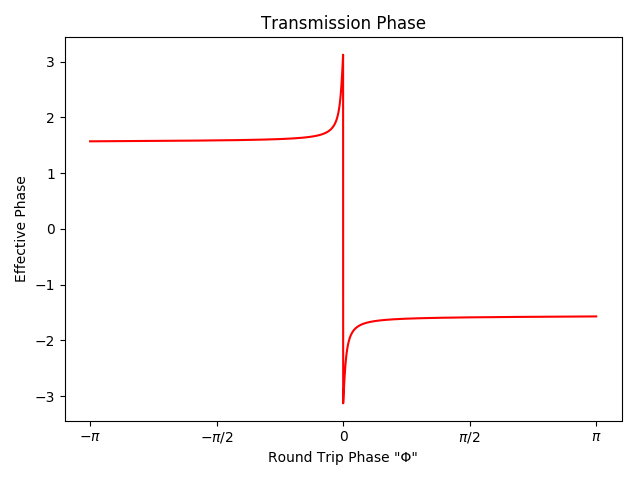
\includegraphics[width=0.5\textwidth]{Phase_trans_FP.png}
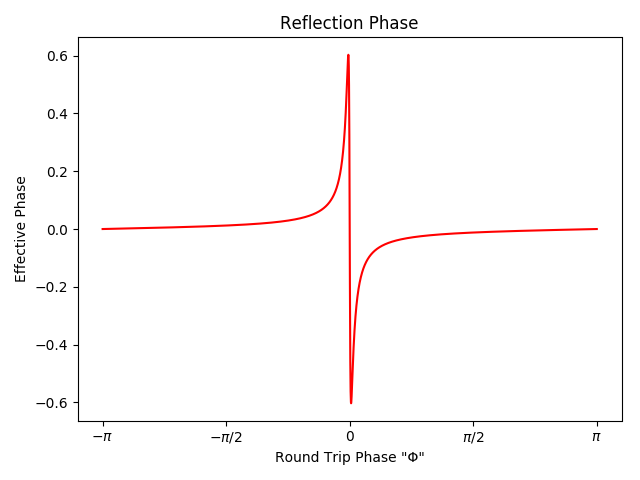
\includegraphics[width=0.5\textwidth]{Reflec_Phase_FP.png}
\caption{Transmission and Reflection phase vs normalized detuning of an asymmetric Fabry-Perot resonator critically coupled.}
\end{figure}

The effective phase also called transmission phase of the system, which is the phase acquired upon transmission, gives us the information about the dispersion of the system. It is basically the argument of the complex transmitivity of the resonator (Eq. 2.4). Any complex number, $z = x + iy$, can be written as $z = |z|exp(i\phi)$. Where, $\phi$ is the argument of the complex number $z$ given by $\phi = tan^{-1}(y/x)$. Now we can write for our complex transmitivity as,

\begin{align*}
\tau = \frac{E_{t}}{E_{i}} = |\frac{E_{t}}{E_{i}}|\,exp(i\phi_{eff})
\end{align*} 

Where,

\begin{equation}
\phi_{eff} = arctan(\frac{Im[\tau]}{Re[\tau]})
\end{equation}

\subsection{Phasor Plots}
Phaser plots are another useful way to study the behavior of light inside the optical cavity. The phasor plots are the complex plots between Real and Imaginary parts of the complex reflectivity and transmitivity (equation 2.3 and 2.4 respectively). Figure 2.4 shows the phasor plots of both transmitivity and reflectivity of an asymmetric Fabry-Perot resonator over the detuning period of 0 to $2\pi$ radians. 

\begin{figure}[h]
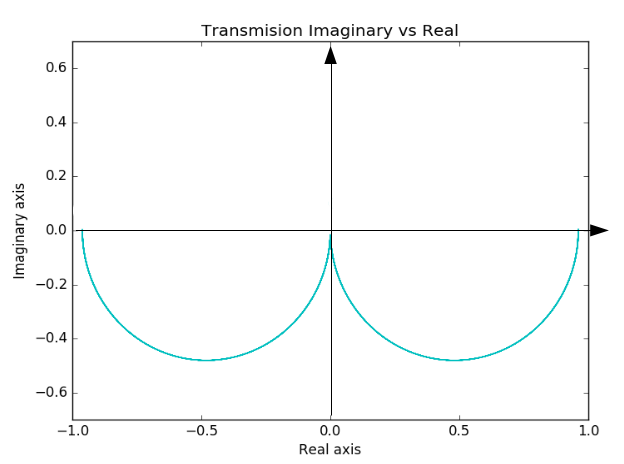
\includegraphics[width=0.5\textwidth]{Trans_ImagvsReal_Phaser.png}
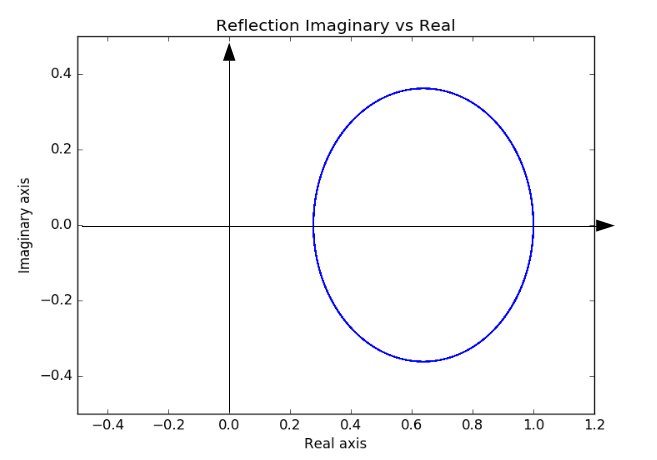
\includegraphics[width=0.5\textwidth]{Reflection_ImagvsReal_Phaser.png}
\caption{Phaser plots of complex Transmitivity and Reflectivity of an asymmetric Fabry-Perot resonator from 0 to $2\pi$}
\end{figure}

\subsection{Finesse, Q-factor}
\subparagraph{\normalfont \large The resonance condition is fulfilled when the (compelling) circumference of the ring, or for the most part the round-trip length, is equivalent to a whole number numerous of the optical wavelength inside the medium. This means a progression of Lorentzian-molded transmission bends equally dispersed in recurrence by the FSR (Free Spectral Range), with the resonance linewidth portraying the capacity time of photons inside the cavity. The photon lifetime can be standardized to one optical cycle, known as the quality factor (${\mathcal Q}$), or the cavity round-trip time, known as the cavity Finesse (${\mathcal F}$). The most extreme reachable Q-factor is characterized as ${\mathcal Q_{int}}$, which is the intrinsic loss of the cavity such that, ${\mathcal Q_{int}} = 2\pi\,n/(\alpha_{i}\,\lambda_{res})$ [16] where $\alpha_{i}$ is the intrinsic loss coefficient and $\lambda_{res}$ is the free-space resonant wavelength.  At the point when the resonator is coupled to the outer world, the Q-factor further decreases because of the loss imported by the coupler (${\mathcal Q_{ext}}$). This Q-factor, which defines mostly coupling and related external losses, can be given by ${\mathcal Q_{ext}} = (2n \pi L)/ {\lambda_{res}\, T}$, where $L$ is the circumference of the resonator (in case of a ring), $\lambda_{res}$ is the resonant frequency, and $T$ is the transmitivity coefficient. Thus the total quality factor ${\mathcal Q_{load}}$ is comprised of these two parts: ${\mathcal Q_{load}^{-1}}$ = ${\mathcal Q_{int}^{-1}}$ + ${\mathcal Q_{ext}^{-1}}$.}

\begin{align*}
{\mathcal F}inese = \frac{2 \pi}{\gamma} \\ 
\\
{\mathcal \gamma} = \frac{4}{\sqrt{F}} \\
\\
F = (\frac{2r}{1-r})^{2} 
\end{align*}

Thus,

\begin{equation}
{\mathcal F}inese = \frac{\pi \sqrt{F}}{2}
\end{equation}

Similarly, 

\begin{align*}
{\mathcal Q}_{factor} = \frac{\lambda_{res}}{FWHM} \\ 
\\
{\mathcal Q}_{factor} = \frac{nLf}{\lambda}
\end{align*}
\begin{equation}
{\mathcal Q}_{factor} = m f
\end{equation}


\section{Ring Shaped Resonators}
Optical interferometers such as Fabry-Perot or Gires-Tournois resonators are extremely useful in making devices that are compatible in making spectroscopy tools, add-drop filters for specific optical frequencies, laser cavities as well as dispersion compensators. Due to their free space structural design, they are quite incompatible with planar integrated technology. Thus, we require another geometry of devices which have similar spectral properties. These can be fabricated easily and effectively on microchips and waveguiding geometries by molding of different waveguides into a ring shape.

Let us now discuss how ring resonators, whose principle is pretty much similar to the Fabry-Perot resonator and are more simple to make, operate. Basically, a ring resonator is a simple waveguide which is turned in to the shape of a ring (see Fig. 2.5). This allows it to exhibit resonant behavior on very specific frequencies.


\subsection{Evanescent Coupling}
The optical systems discussed above experiences the passage of light across the ring from the optical waveguide through a process known as evanescent coupling. Evanescent coupling is a classical phenomenon whose quantum interpretation is exactly as photon tunneling. It is basically the power transfer of the wave which is directly dependant on the proximity of the bent waveguide and from the straight waveguide. Also, the length or area that has been exposed to the coupler also plays an important role in i.e. how many area of the waveguide/resonator overlaps; illustrated in Fig. 2.5.
\subparagraph{\normalfont \large Coupling strength of an ideal coupler is dependant on the interaction length between the two optical modes which means that the power will transfer more efficiently when the two modes are matched on the basis of their respective phases. This allows us to observe distinct behaviors as well as multiple resonances in transmittance and reflectance.} 

\begin{figure}[h]
\centering
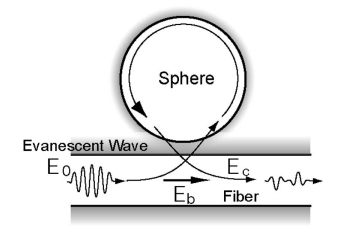
\includegraphics[width=0.50\textwidth]{evanescent_wave.png}
\caption{Schematic illustration of the microsphere-fiber-taper
system [2].}
\end{figure}

\subparagraph{\normalfont \large The light is coupled inside the ring due to two sets of coupling approaches, one being lateral and other being vertical. Either one of these two approaches is necessary for the light from the optical waveguide to couple inside the bent waveguide (ring). The light stays, or resonates, inside the bent waveguide due to the effect of total internal reflection. Lateral coupling requires the same plane fabrication of waveguide and bent waveguide which are easier to fabricate. To ensure strong coupling, small separation is required between the waveguide and bent waveguide. Lateral configuration requires a single layer only but very accurate lithography and etching processes must be done to open up the gaps between straight and ring waveguides with high precision. In vertical coupling transport and bent waveguides are etched in various layers. Vertical coupling expels the index contrast restriction of lateral coupling, additionally, it is an empowering innovation for the ring radii less than $ \approx5 \mu m$. Another bit of leeway of the vertical arrangement is that the ring and waveguide layers don't need to be a similar thickness, which improves the design opportunity.}


These resonators, when fabricated on the chip, display different effects of coupling and transfer of wave energy. These kinds of behaviors have been noticed in all kind of classical waves, such as sound waves, which was first observed inside a large cathedral's halls, thus it was named whispering gallery modes [4]. Also, these resonators can be made using different material but in the scope of this thesis, we used semiconductor silicon as the primary material. 


\subsection{Coupling Regimes}

The transmission spectrum of the waveguide-ring coupled system now depends on the proximity and coupling effects. Let us discuss different coupling conditions for these resonators. Fig. 2.6 shows plots for an all-pass resonator for under, over, and critically coupled system and also for a lossless all-pass system.

\begin{figure}[h]
\centering
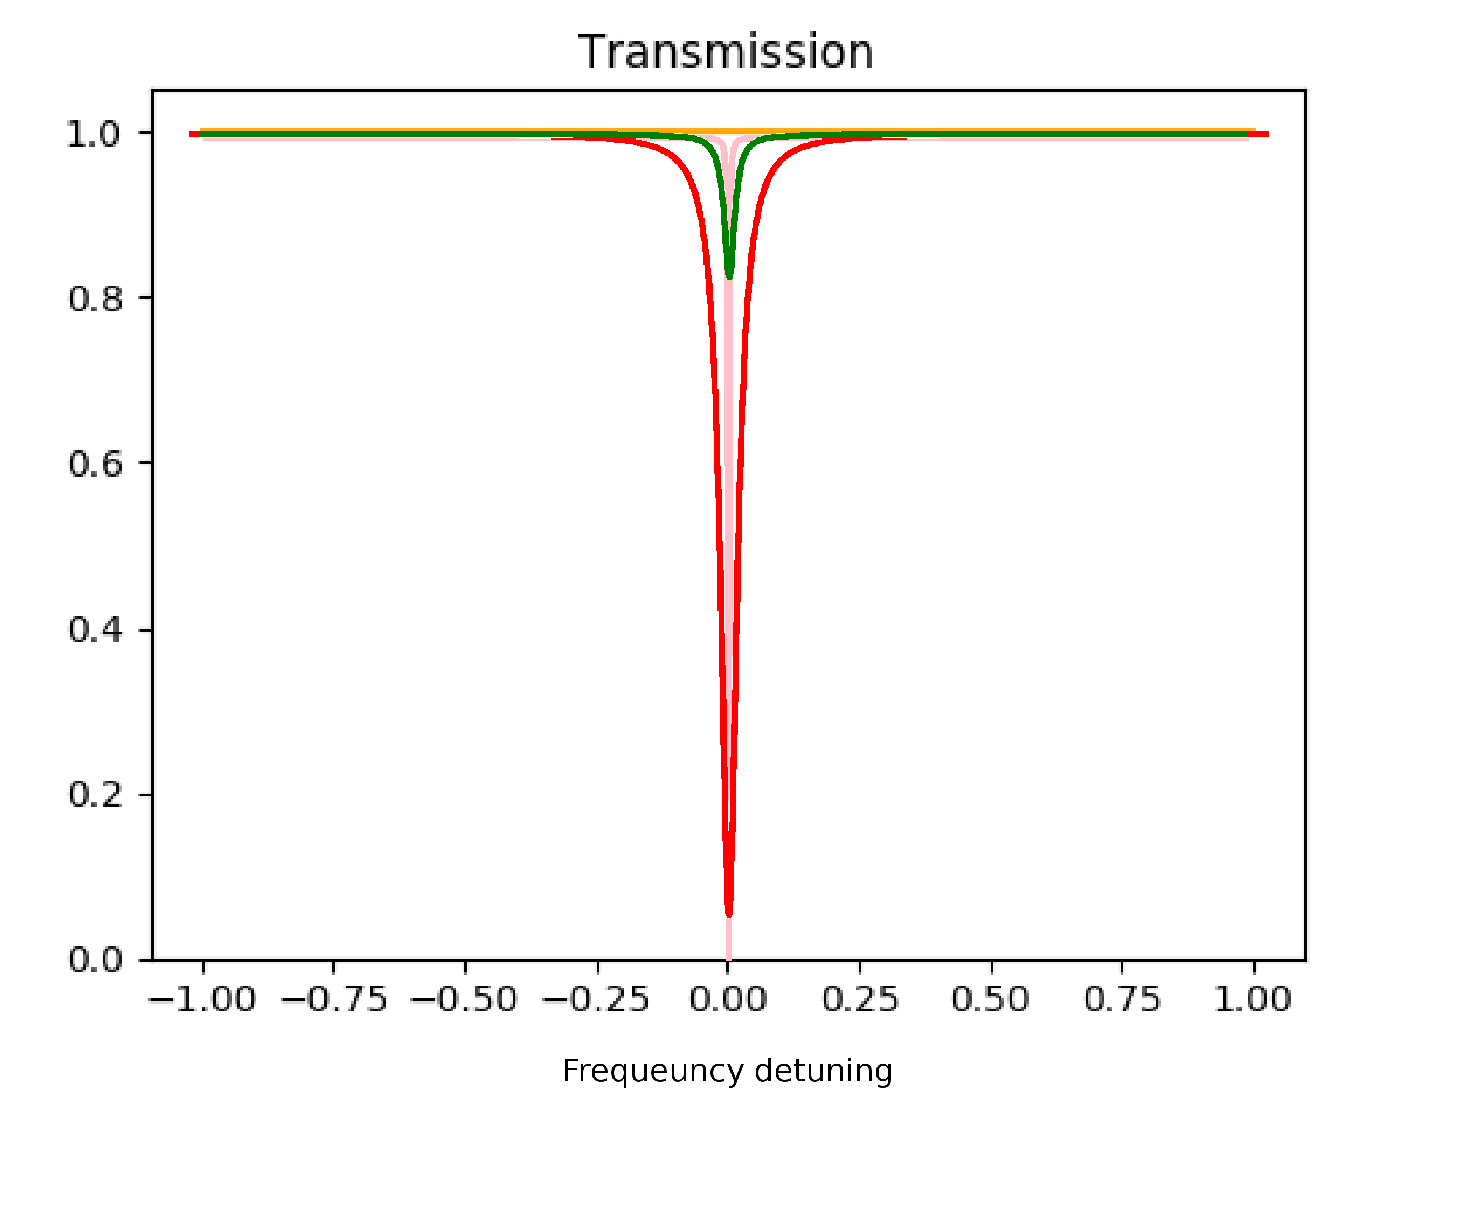
\includegraphics[width=0.5\textwidth]{under_over_couple.eps}
\caption{Different couplings shown in different colors.}
\end{figure}

Light when couples inside the ring will lose some part of its intensity. The amount of light that travels inside the ring will acquire a phase shift by completing one round trip and will now interfere destructively with the light which was not coupled inside the resonator. If the phase shifted light has amplitude weaker than the original or uncoupled light, the regime will be known as under-coupled. If the amplitude is higher than the original pulse, the regime would be over-coupled. Similarly, when the amplitude matches exactly with the outside light, the regime would be known as critically coupled. Also, if the light passes through the system without any attenuation or loss, we get $100\%$ transmission.


\section{Gain Incorporation in Resonators}
Light, when travels through a medium, loses its intensity exponentially. This effect can be explained by Beer's Law for electromagnetic intensity. But some mediums, whose refractive index is such as they oppose the exponential decay of the light and rather increase the intensity in the propagation through the medium, are called natural gain medium. Also, there can be an artificial source to activate gain in a certain system. This is done by pumping energy or external light source i.e. Lasers, to excite the atoms inside the cavity. This makes the stimulated emission releases of the photons increase exponentially and we see an increase in the incident intensity of the input light. We can use these gain mediums and build micro-resonators from them and observe different quantum optical phenomenons. First I will explain a bit about how gain works.


\subsection{Beer's Law}
The simple radiation law follows the beer's law in the absorption of any kind of radiation inside a medium. This tells us that the initial intensity of the light source depends on the variables of the medium it is passing through. For electromagnetic radiation, we can write this law as,

\begin{equation}
I(z) = I_{o}\exp(-\alpha z)
\end{equation}

Here, $I_{o}$ is the initial intensity of the radiation, $\alpha$ is the attenuation constant of the medium, $z$ is the amount of distance traveled through the medium and $I(z)$ is the intensity of light after traveling the distance $z$.

\begin{figure}[h]
\centering
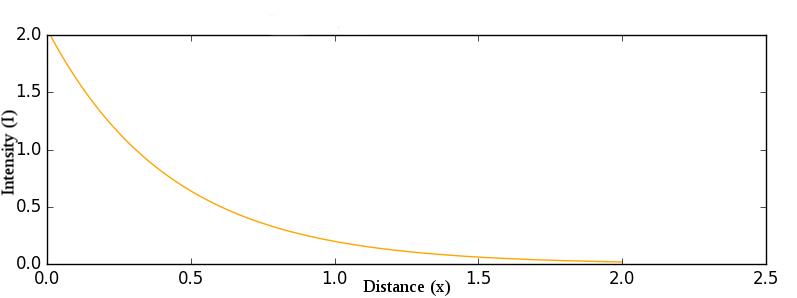
\includegraphics[scale=0.75]{beer's_law_withoutgain.png}
\caption{Beer's law plot with attenuation 0.01/cm: y-axis shows the intensity of light and x-axis shows the distance traveled in meters.}
\end{figure}


\subsection{Beer's Law in Presence of Gain}
In a gain medium, the intensity of the light will not decrease but it will gradually increase. This means that the attenuation $\alpha$ is negative or we can introduce a new coefficient for such medium say $g$ such that $-\alpha \to +g$ where $g$ is some positive real number. This means that the intensity function now grows exponentially rather than decaying exponential.

\begin{equation}
I(z) = I_{o}\exp( +g z)
\end{equation}

\begin{figure}[h]
\centering
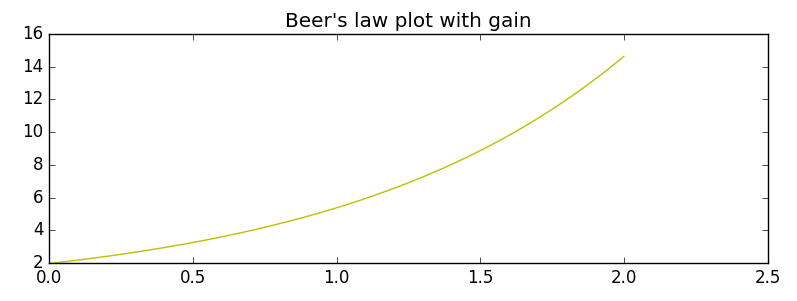
\includegraphics[scale=0.75]{beer's_law_withgain.png}
\caption{Beer's law plot with gain value 0.01/cm: y-axis shows the intensity of light and x-axis shows the distance traveled in meters.}
\end{figure}

\subsection{Gain Medium}
The active laser medium also called gain medium or lasing medium is the source of optical increase inside a laser. The gain is the result of stimulated emission of electronic or sub-atomic changes to a lower energy state from a higher energy state recently populated by a pump source. This gain in optical systems is usually used for amplification purposes and hence make optical amplifiers. Certain crystals, typically doped with rare-earth ions (e.g. neodymium, ytterbium, or erbium) or transition metal ions (titanium or chromium) can be used as a gain medium. Also, Semiconductors, e.g. gallium arsenide (GaAs), indium gallium arsenide (InGaAs), or gallium nitride (GaN) can also be used when doped [14]. Also, some material such as liquids in the form of dye solutions as used in dye lasers can also be used to make a gain element for active resonators [15].


\section{Group Delay and Group Advance}
The velocity of light is a universal constant $c \approx 299792458 m/s$ in free space. However, the light velocity depends upon the medium when it propagates through it. The medium's dispersive properties are defined by the refractive index $n$ of the material. The light pulse propagating from this material experiences delay in the arrival time as compared to the arrival time in a vacuum. 
To comprehend the results of scattering from the refractive index, we initially think about the proliferation of monochromatic light emission through a material. The phase velocity ($v_{p}$) depicts the speed at which the wavefronts travel through the material and is given by: $v_{p} = c/n $ . Thus when the light pulse propagates through the medium, different wavlengths of the wave travels at different speeds because $n$ is a function of frequency $\omega$. Here, group index is put into account due to the collective effects upon the wave packets of different frequencies, which is given by:
\begin{align*}
n_{g} = n + \omega\frac{dn}{d\omega}
\end{align*}

Here, $n_{g}$ is the group index of the material and $\omega$ is the frequency of the wave. Thus now we can define the group velocity of the propagating wave, which is the speed at which the envelope of the incoming pulses moves through the dispersive medium, given by:
\begin{align*}
v_{g} = \frac{c}{n_{g}}
\end{align*}

Thus the light experiences reduction in its velocity inside a dispersive medium. If the value of $n_{g} \approx 10^{8}$, then we experience ultra slow velocities of light which are measured up to $8m/s$ [17-19]. If group index becomes less than 1, such that $n_{g} < 1$, then we observe group velocities greater than the speed of light in vacuum, such that, $v_{g} > c$. This does not violate Einstein's Theory of Relativity [20] because there exist various proposals [5–8] for observing such effects by using anomalous dispersion near an absorption or gain lines [7-8]. The group index can also become negative, such that $n_{g} < 0$, resulting in negative group velocities which are sometimes also referred as `Backward light' because it appears to propagate backward in the medium. We can understand the negative group velocity by having a medium of length $d$, so it will take $d/v_{g} = n_{g}d/c$ amount of propagation time for a light pulse to cross it. And the vacuum transition time would be $d/c$, thus the time delay would be $\Delta T = d/v_{g} - d/c$ which can be written as, $(n_{g}-1)d/c$. So for negative values of $n_{g}$, the delay time $\Delta T$ is negative which results in group advancement. This concept can be perceived as that if the light pulse is incident on such medium, the light pulse would appear on the other side sooner than if it had traveled through a vacuum. Figure 2.8 illustrates the propagation through a negative index medium [9]. 

\begin{figure}[h]
\centering
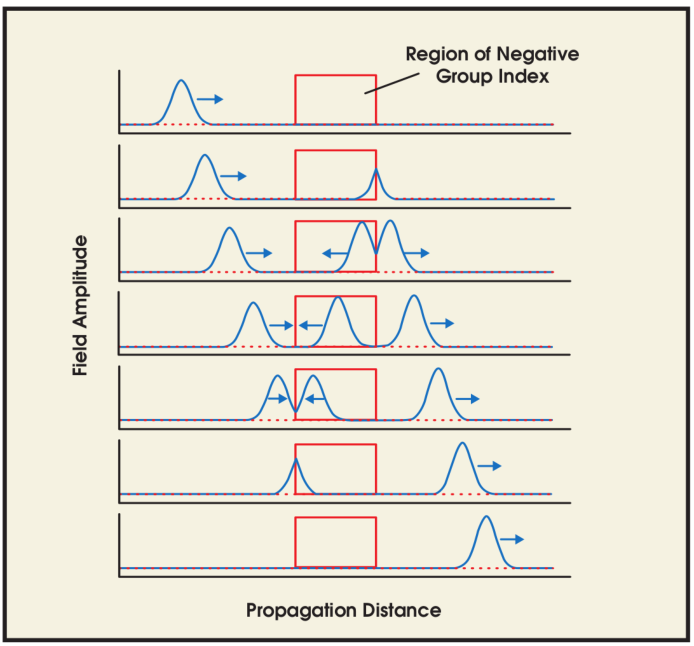
\includegraphics[scale=0.75]{negative_vg_pic.pdf}
\caption{Time intervals of a wave propagating through a negative index material. Notice that the peak of entering pulse leaves before it enters the system.}
\end{figure}

The slow light propagation of light is enhanced by EIT which is a transparency window in the absorption line of the system. Slow light can be used in optical buffers where controllable slow light can dramatically increase the system's performance. Also, the spectral sensitivity of an interferometer [11] can be highly enhanced by introducing a slow-light medium, as well as slow light has a large number of uses in defense applications. Fast light, on the other hand, can be used to make ultra-sensitive gyroscopes [12] and gravitational wave detectors in the fields of astrophysics [13].



\section{All-Pass Ring Resonator}
A straightforward ring resonator is made by taking one yield of a conventional directional coupler and bolstering it once again into one input. Such a device displays periodic cavity resonance (reverberation) when light navigating the ring procures a phased move relating to a number numerous of 2$\pi$ radians. The resonator is numerically defined from two parts: a coupling quality and an input way. In opposition to the limitless entirety inferences performed before for the Fabry– Perot and Gires– Tournois, in which we expected steady-state task and coordinating fields and derived basic spectral properties. Although both strategies are similarly substantial, the field-coordinating technique has the benefit of simplicity.
\begin{figure}[h]
\centering
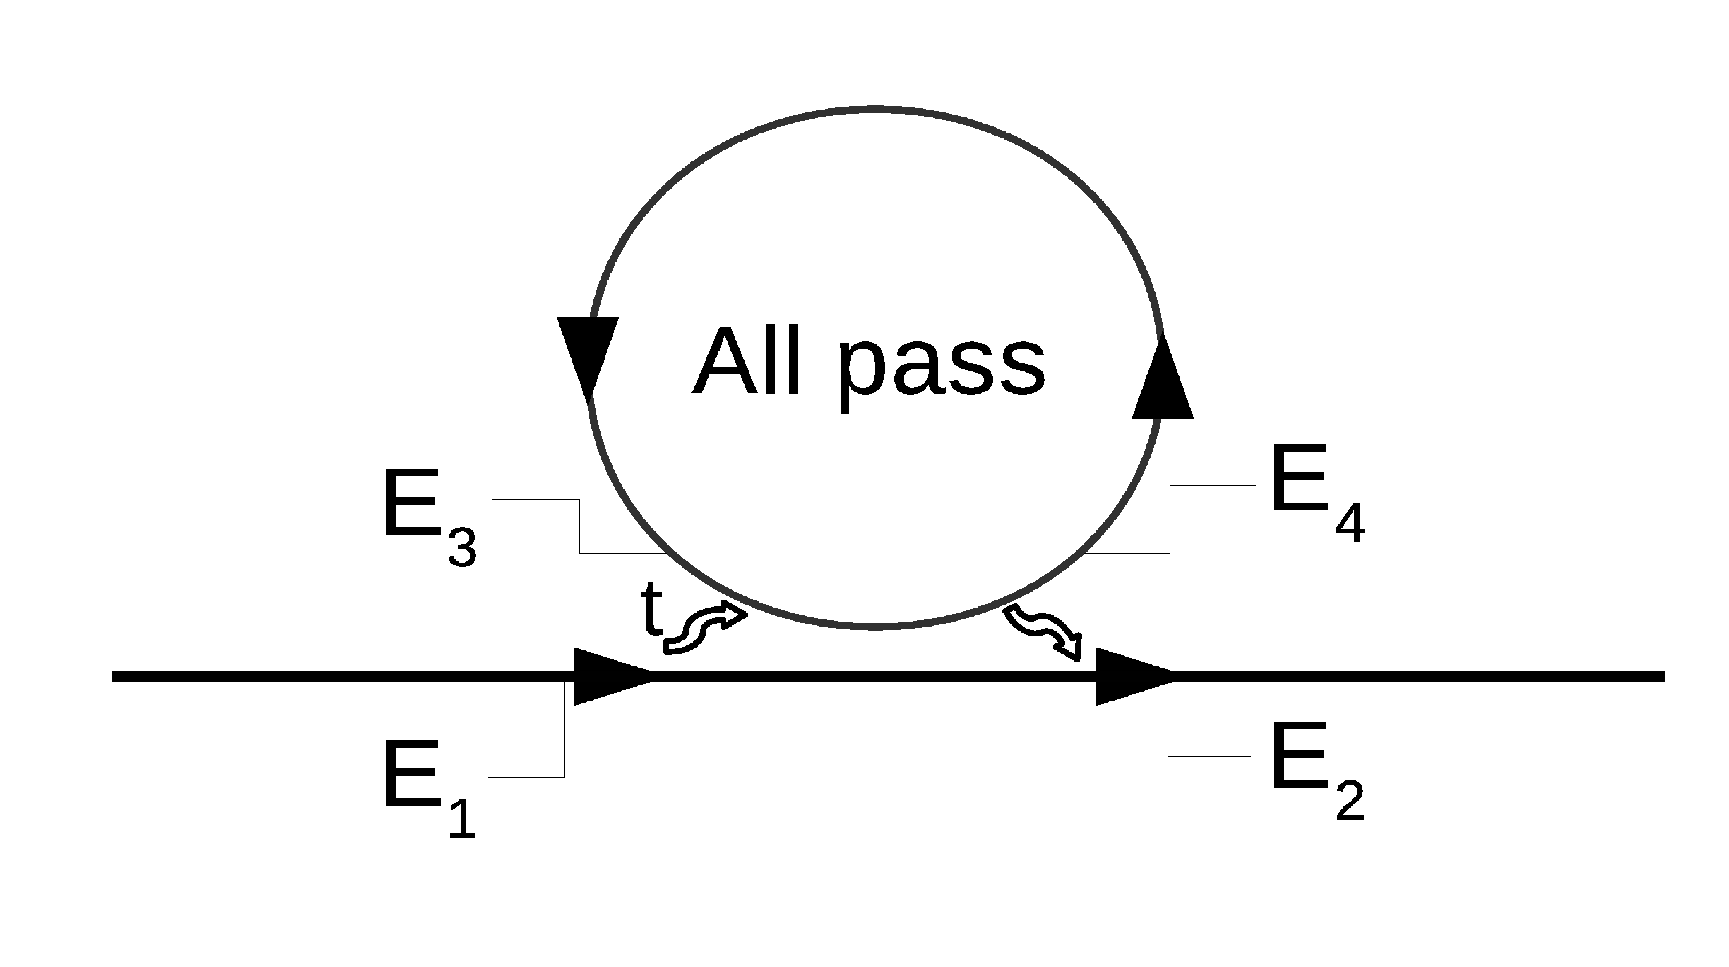
\includegraphics[width=0.85\textwidth]{all_pass_resonator.eps}
\caption{Illustrated fields of an all-pass resonator}
\end{figure}

Fig. 2.9 illustrates the basic geometry of the all-pass ring resonator with its respective energies. The incoming input power is $E_{1}$, which couples inside the ring through the evanescent coupling. Then it travels as energy $E_{4}$ and makes a round trip phase. If this phase matches with the input signal, it makes constructed interference with the incoming light with energy $E_{3}$ and transfers its energy to the optical waveguide again with energy $E_{2}$. The complex transmitivity and reflectivity are given by equation 2.10, as the reflection is not considered in this geometry.
 

\begin{equation}
\frac{E_{t}}{E_{i}} = \frac{r - a_{1} e^{i\phi_{1}}}{1 - r a_{1} e^{i\phi_{1}}}
\end{equation}

Here, $r$ is the self-coupling coefficient, $a = e^{-\alpha L/2}$ is the intrinsic loss for circumference $L$ and attenuation $\alpha$, and $\phi = \omega T$ is the round trip phase of the ring or single pass phase shift.

\subsection{Transmission of Passive and Active Resonator}
Let us look at the transmission spectra of the passive and active all-pass ring resonator. Fig. 2.10 shows that the transmission peak is changed into a dip as was in the case of a symmetric Fabry-Perot resonator. On the right, it shows when the gain is introduced inside the system, the dip flips into a peak above unity on the graph telling us that we have more transmission on resonant frequencies than the actual input.
\begin{figure}[h]
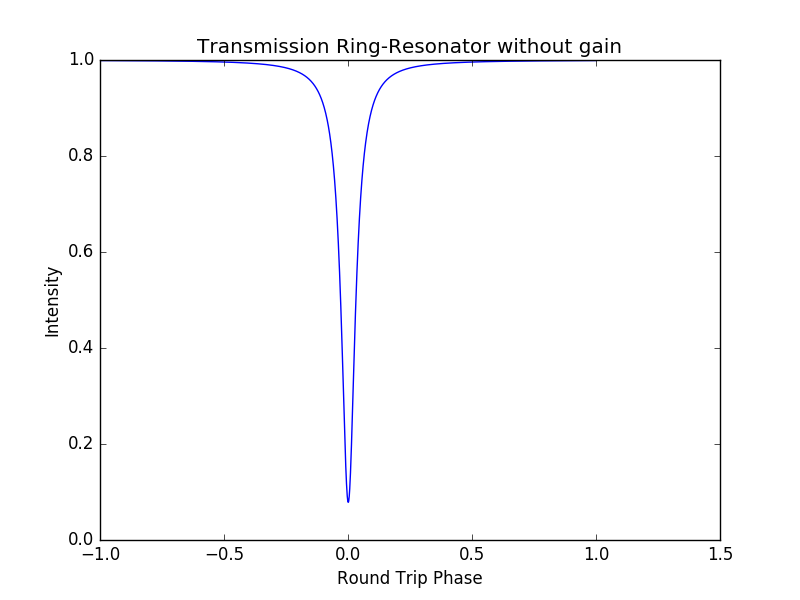
\includegraphics[width=0.5\textwidth]{trans_ring_withoutgain.png}
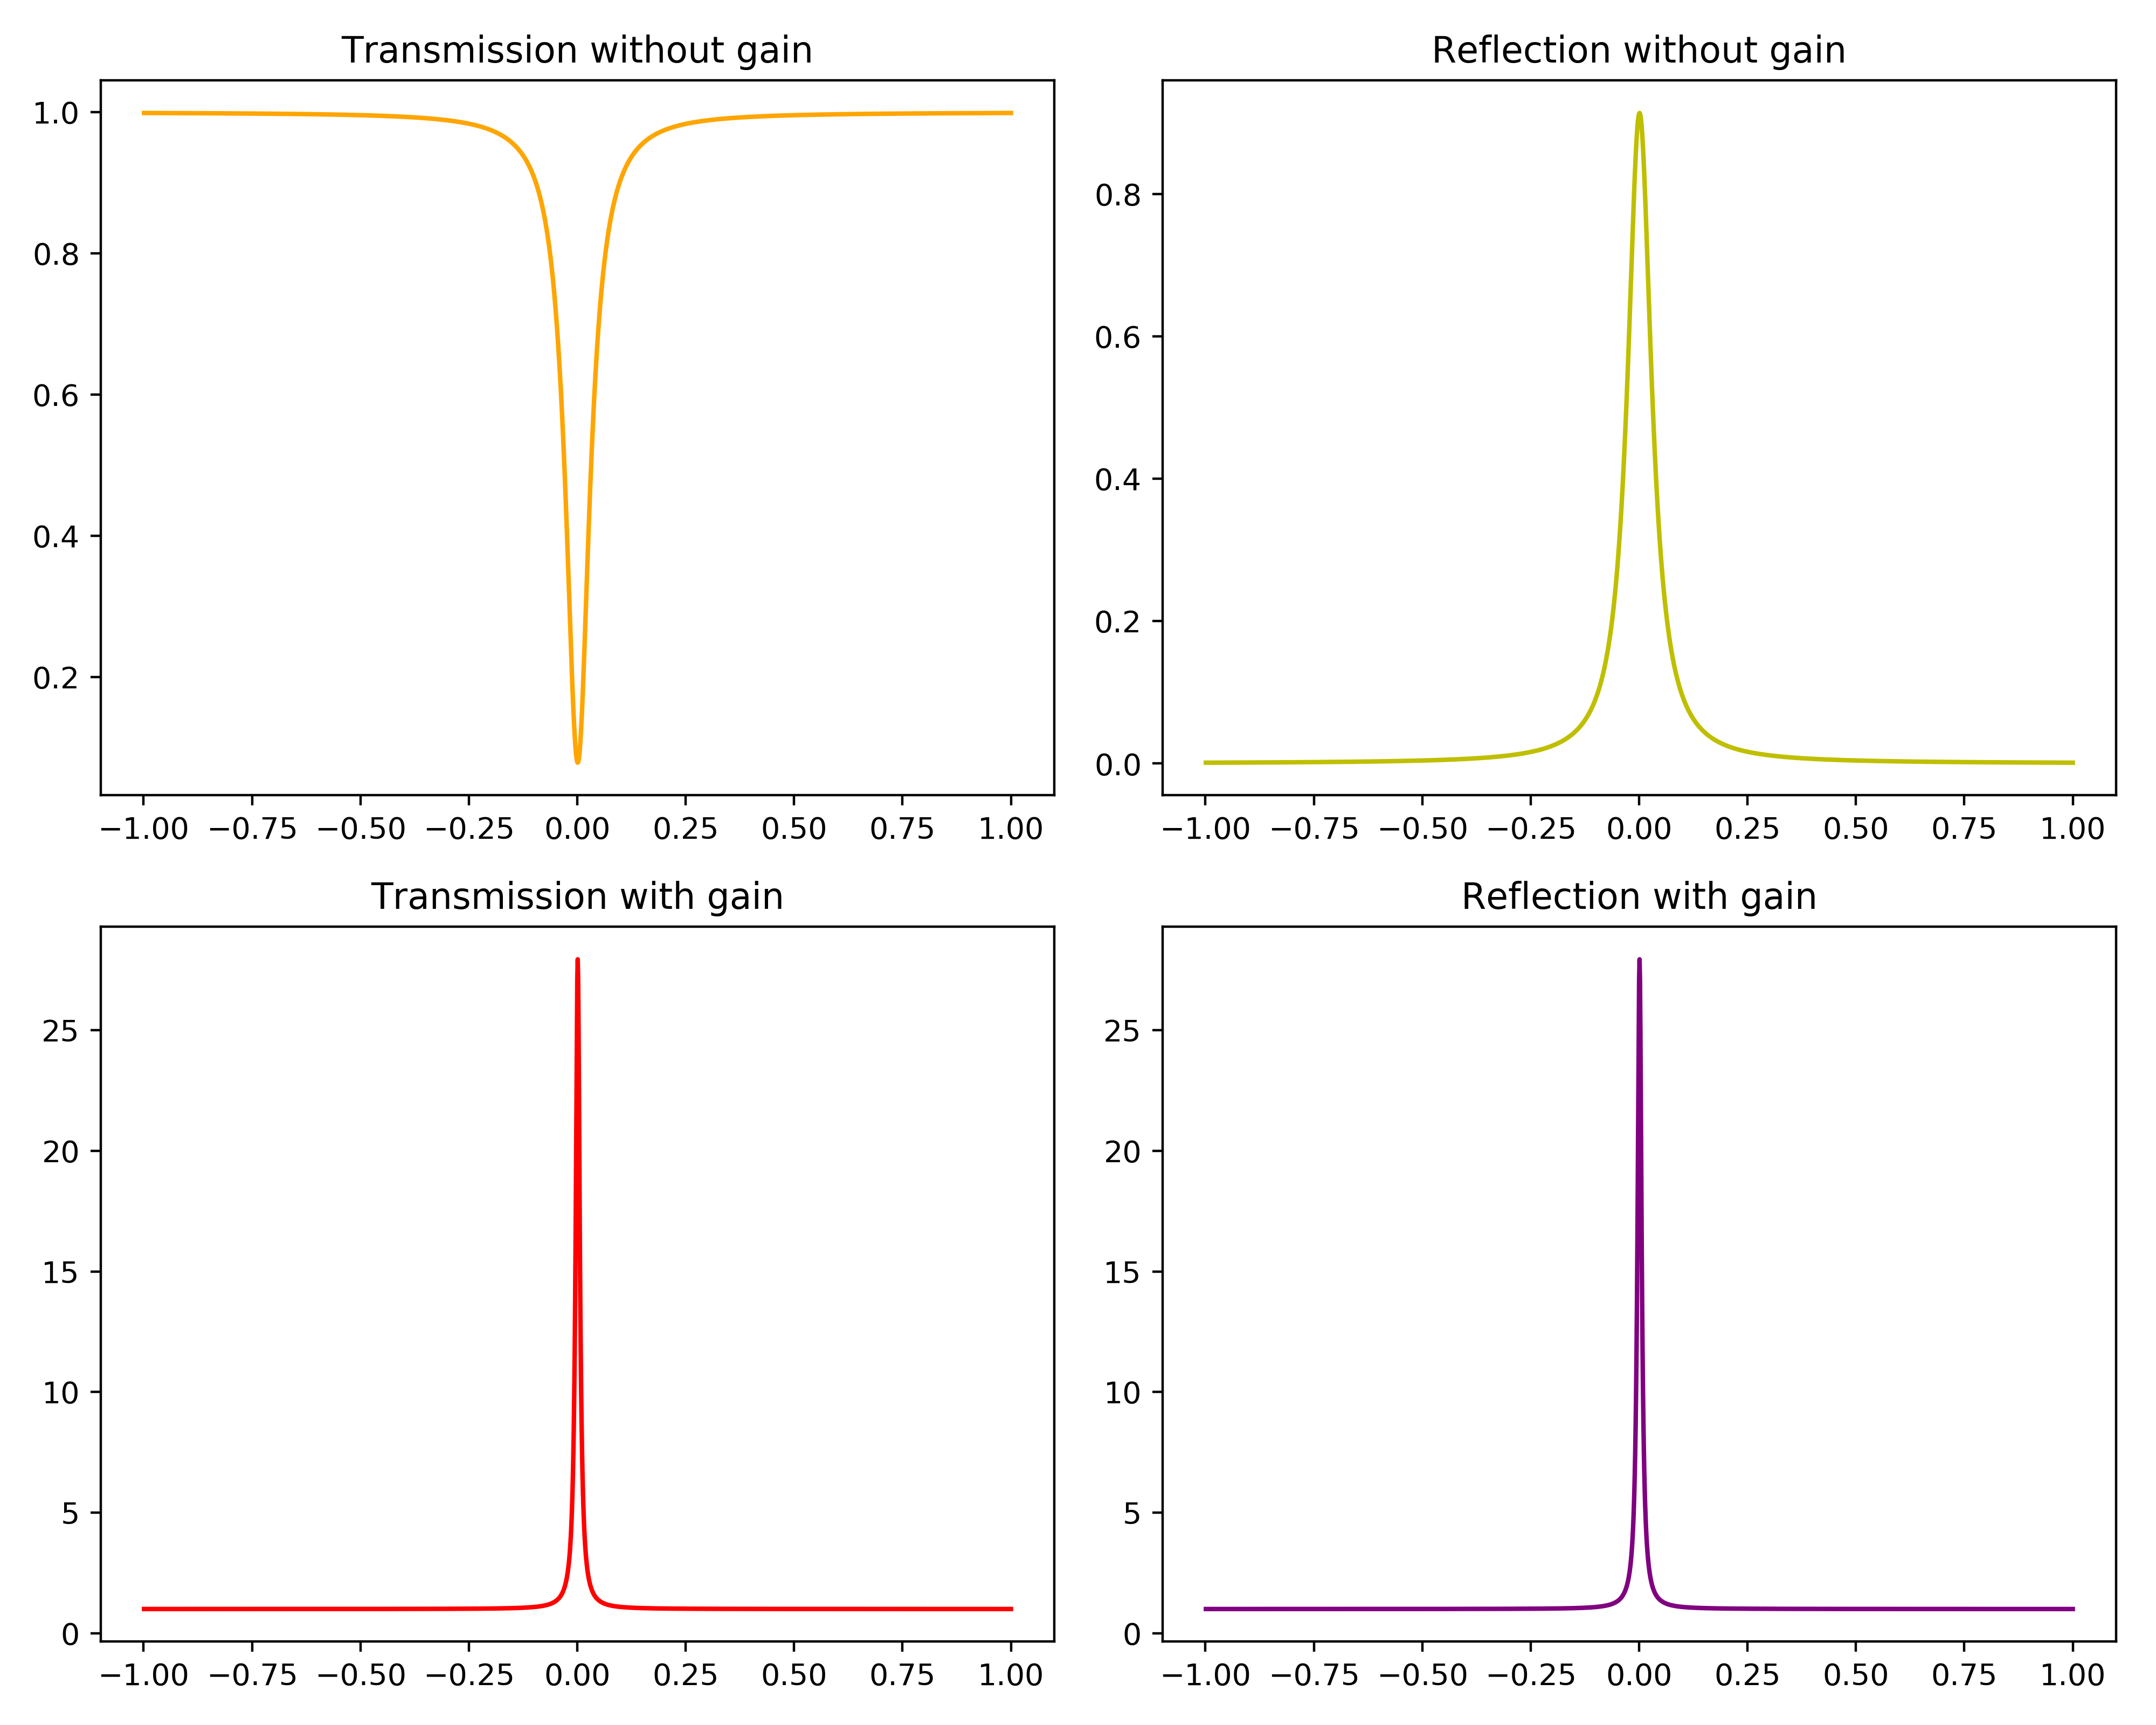
\includegraphics[width=0.45\textwidth]{all-pall_gain.png}
\caption{Transmission spectra of a passive all-pass ring resonator}
\end{figure}


\subsection{Effective Phase}
The phase of the all-pass ring resonator is shown in Figure 2.12. We can easily observe from this that with changing the values of the coupling $r$, the shape of the graph changes as that of a function of $ArcTan(\phi)$. The relation for phase is given by,
\begin{equation}
\Phi_{eff} = \pi + \phi + 2\tan^{-1}\frac{r\sin\phi}{1-r\cos\phi}
\end{equation}

\begin{figure}[h]
\centering
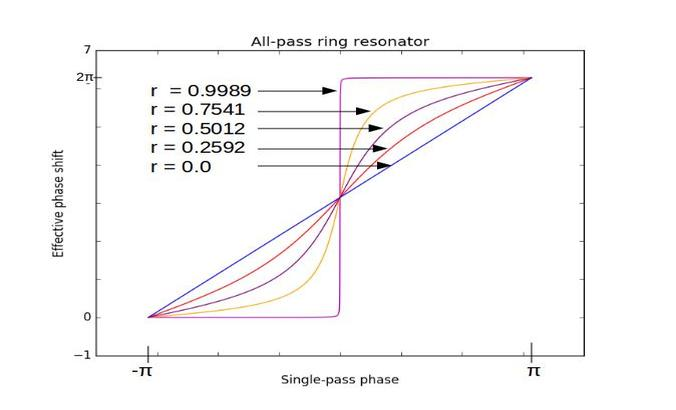
\includegraphics[width=0.65\textwidth]{allpassphase_new.png}
\caption{Phase diagram of an All-Pass ring resonator from 0 to $\pi$ where $r$ is the coupling parameter.}
\end{figure}

\subsection{Phasor Plots}
Now looking into some complex transmitivity of an All-pass ring resonator (Fig. 2.13). This plot is plotted over the complex plain of the detuning limits from 0 to 2$\pi$. 

We observe that the transmission loop does not go to the negative real axis and touches exactly on the origin. The loop cuts the real axis twice on 0 and 1 and is symmetric above and below the axis. 
\begin{figure}[h]
\centering
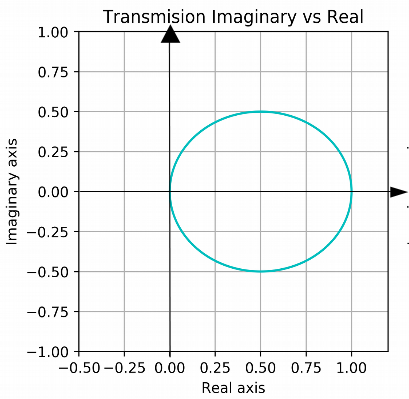
\includegraphics[width=0.5\textwidth]{Imag_vs_real_allpass.png}
\caption{Phaser plot of complex transmitivity of an all-pass ring resonator.}
\end{figure}


\section{Add-Drop Ring Resonator}
The immediate waveguide similarity of a free-space Fabry– Perot is acquired by including a second guide that side-couples to the resonator.
Since this setup acts as a tight band abundancy channel that can include or drop a recurrence band from an approaching sign, it is usually named as an add-drop filter. Fig. 2.14 shows the basic geometry of the add-drop ring resonator with its associated fields labeled accordingly. This resonator has an input, through and drop interfaces where $t_{1}$ is add and $t_{2}$ is drop coefficients. Input field is labeled as $E_{1}$ while the through field is labeled as $E_{2}$. The drop field is on the left top corner labeled as $E_{5}$. The ratio of these fields to the incident/input field defines the total transmitivity and total reflectivity of the filter. The transmission and reflection relations are given in equation 2.12 and 2.13.
\begin{figure}[h]
\centering
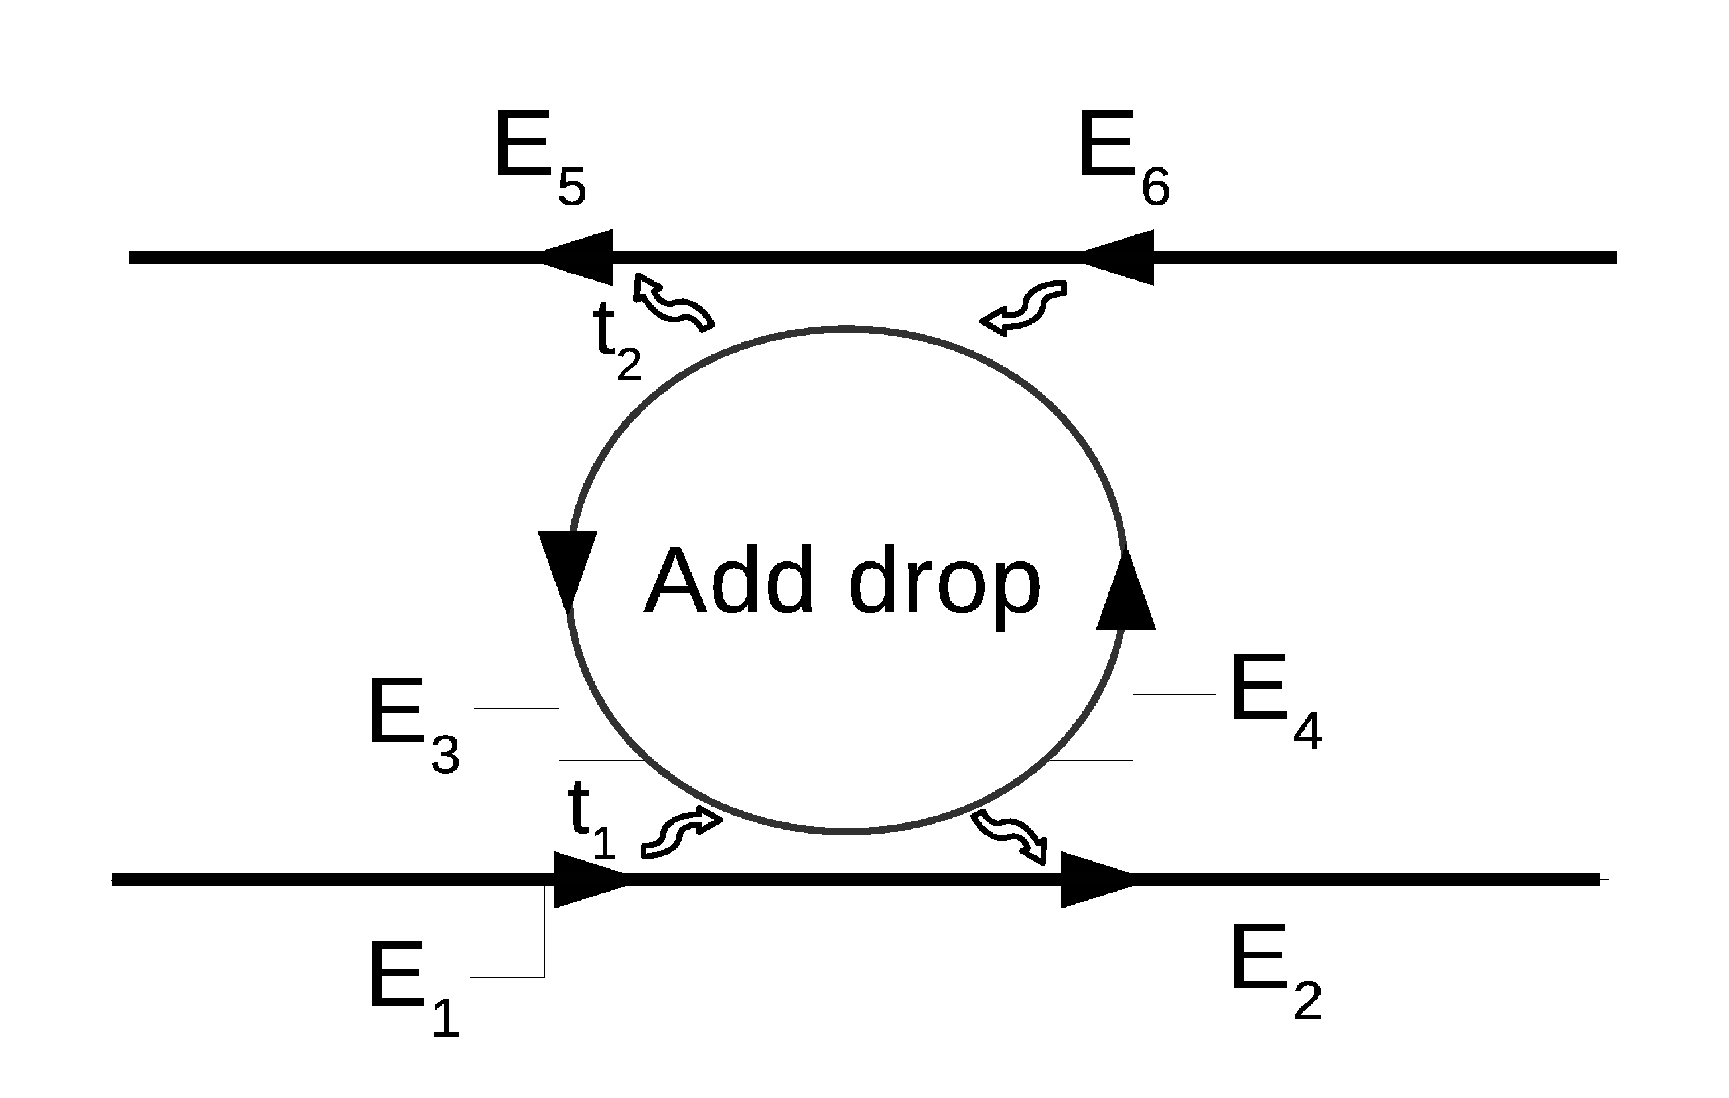
\includegraphics[width=0.70\textwidth]{add_drop_resonator.eps}
\caption{Illustrated fields of an add-drop resonator}
\end{figure}


\begin{equation}
\frac{E_{t}}{E_{i}} = \frac{r_{1} - r_{2} a_{1} e^{i\phi_{1}}}{1 - r_{1} r_{2} a_{1} e^{i\phi_{1}}}
\end{equation}

\begin{equation}
\frac{E_{r}}{E_{i}} = \frac{- t_{1} t_{2} a_{1} e^{i \phi_{1}/2}}{1 - r_{1} r_{2} a_{1} e^{i\phi_{1}}}
\end{equation}



\subsection{Transmission and Reflection}
Let us now look at some reflection and transmission spectra of a passive Add- drop filter. Fig. 2.15 shows that the transmission and reflection peaks are flipped as in case of an asymmetric Fabry-Perot resonator and the transmission phase is a direct function of the detuning. Reflection phase is also shown in Fig. 2.16.

\begin{figure}[h]
\centering
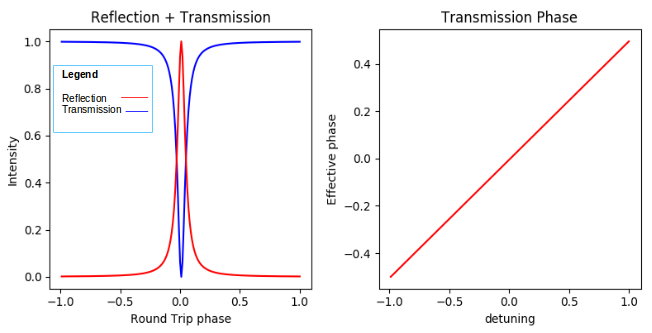
\includegraphics[width=0.5\textwidth]{all_pass_plots_a.png}
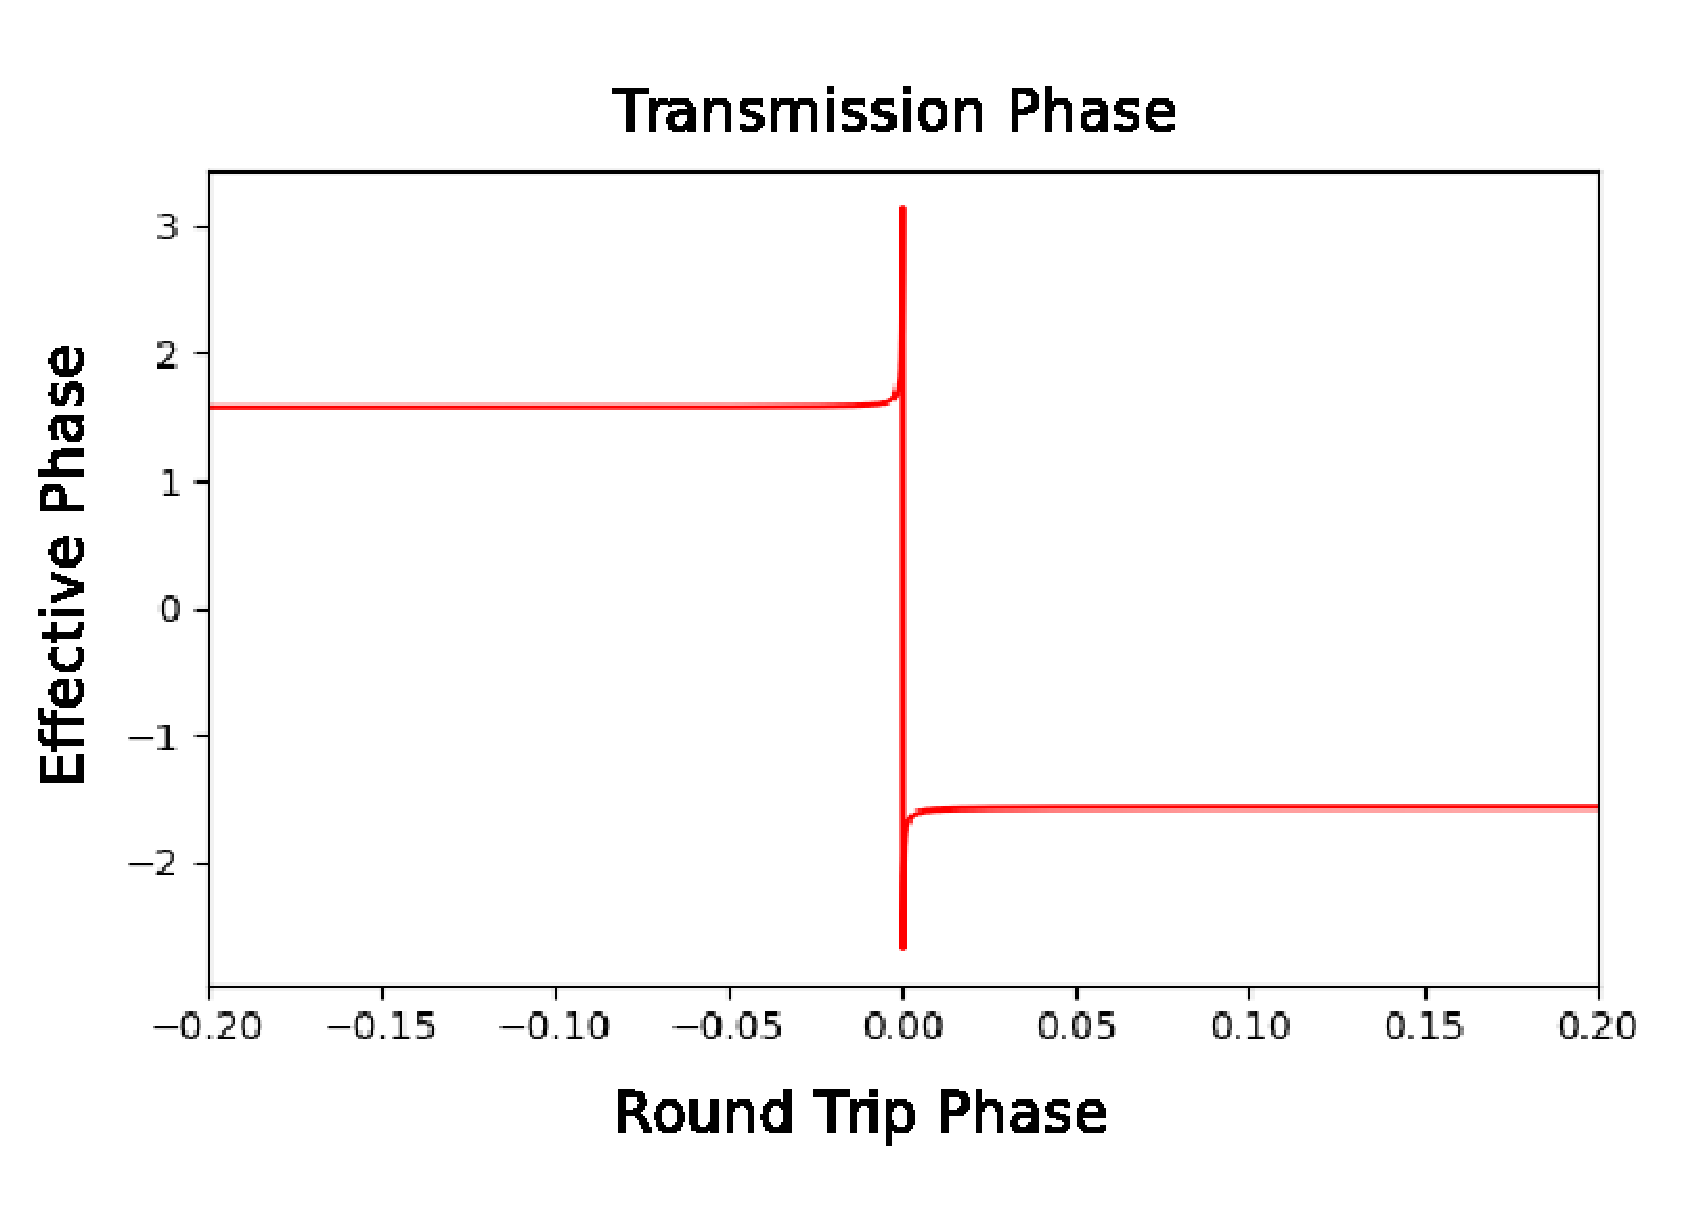
\includegraphics[width=0.5\textwidth]{all_pass_plots_a2.eps}
\caption{Reflection and Transmission spectra along with transmission phase} 
\end{figure}
\newpage
\begin{figure}[t]
\centering
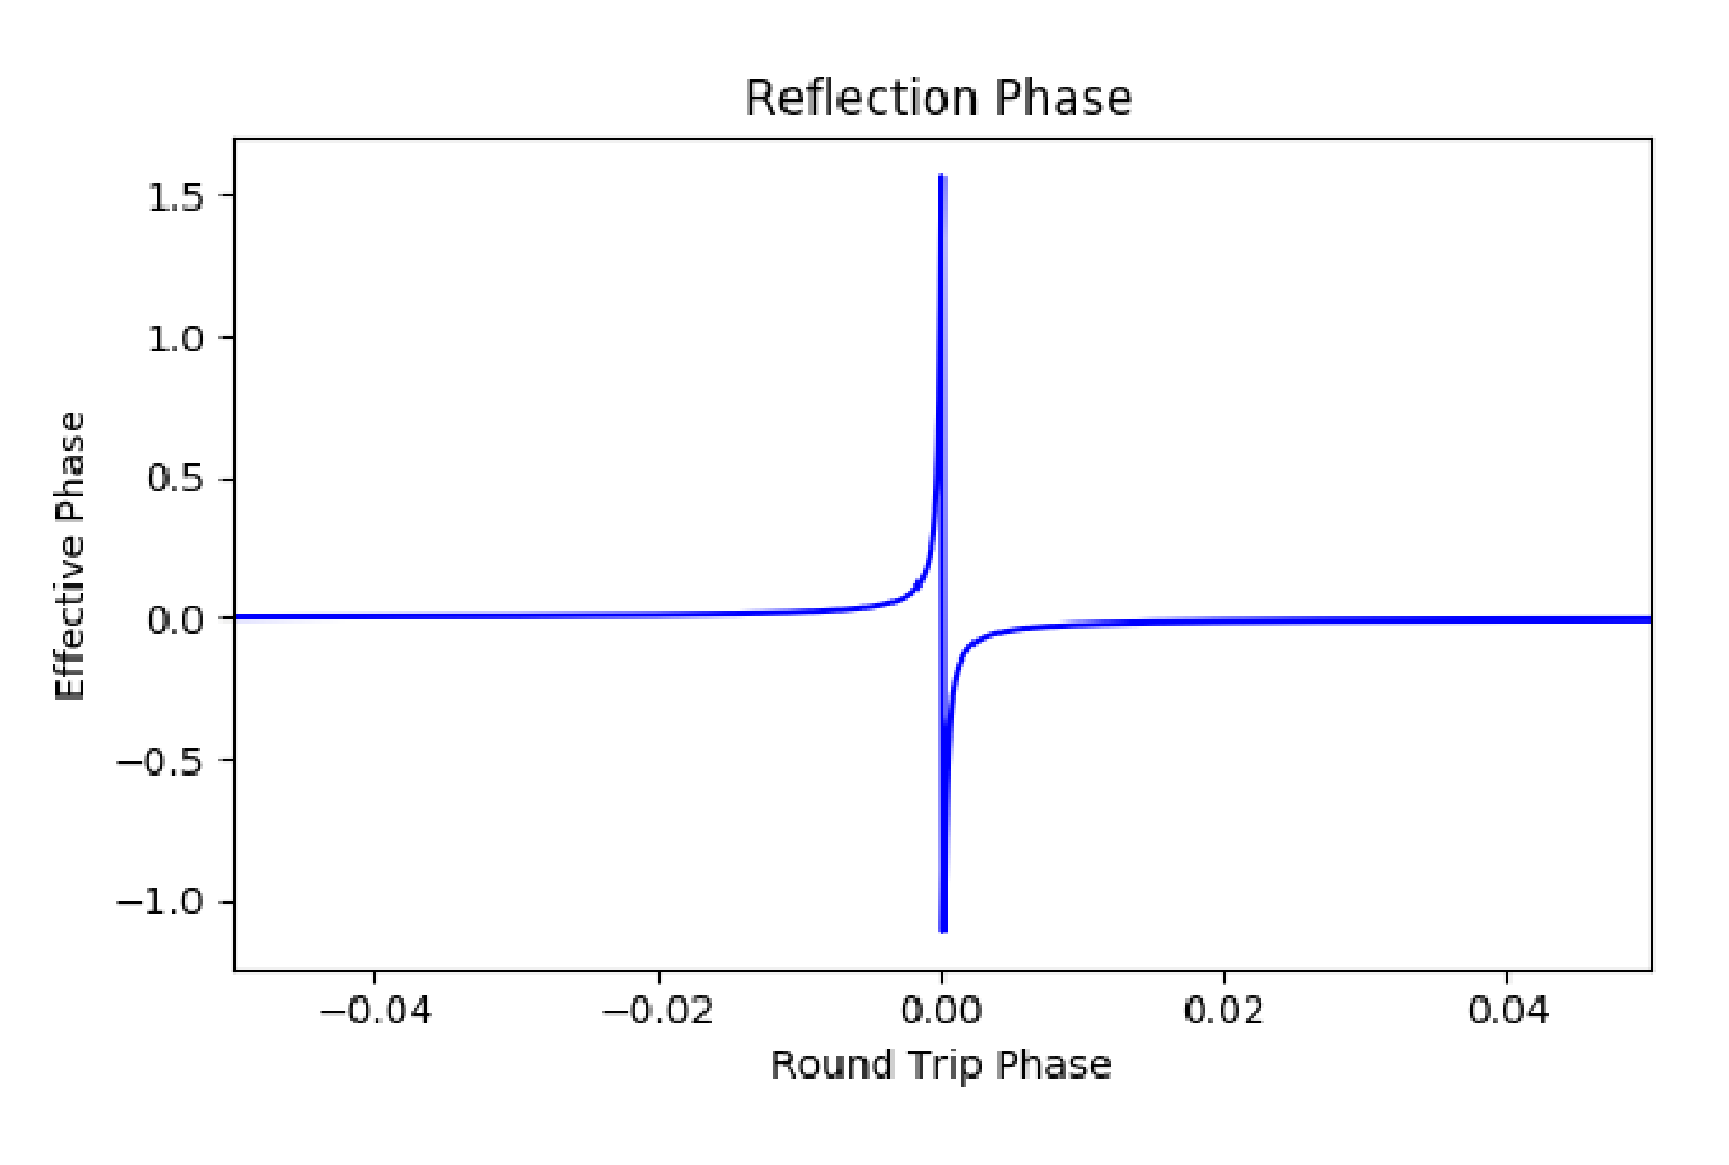
\includegraphics[width=0.5\textwidth]{all_pass_plots_b.eps}
\caption{Reflection phase of the add-drop ring resonator.}
\end{figure}

\subsection{Transmission and Reflection with gain}
Now we introduce gain into the system and observe that the transmission dip also shifts into a peak which above the 1 mark (see Fig. 2.17). Meaning that it is greater than the initial intensity and the reflection peak is almost near zero meaning most of the incident light is being transmitted. We will study the transmission of some other different geometries of ring resonators with gain. 


\begin{figure}[h]
\centering
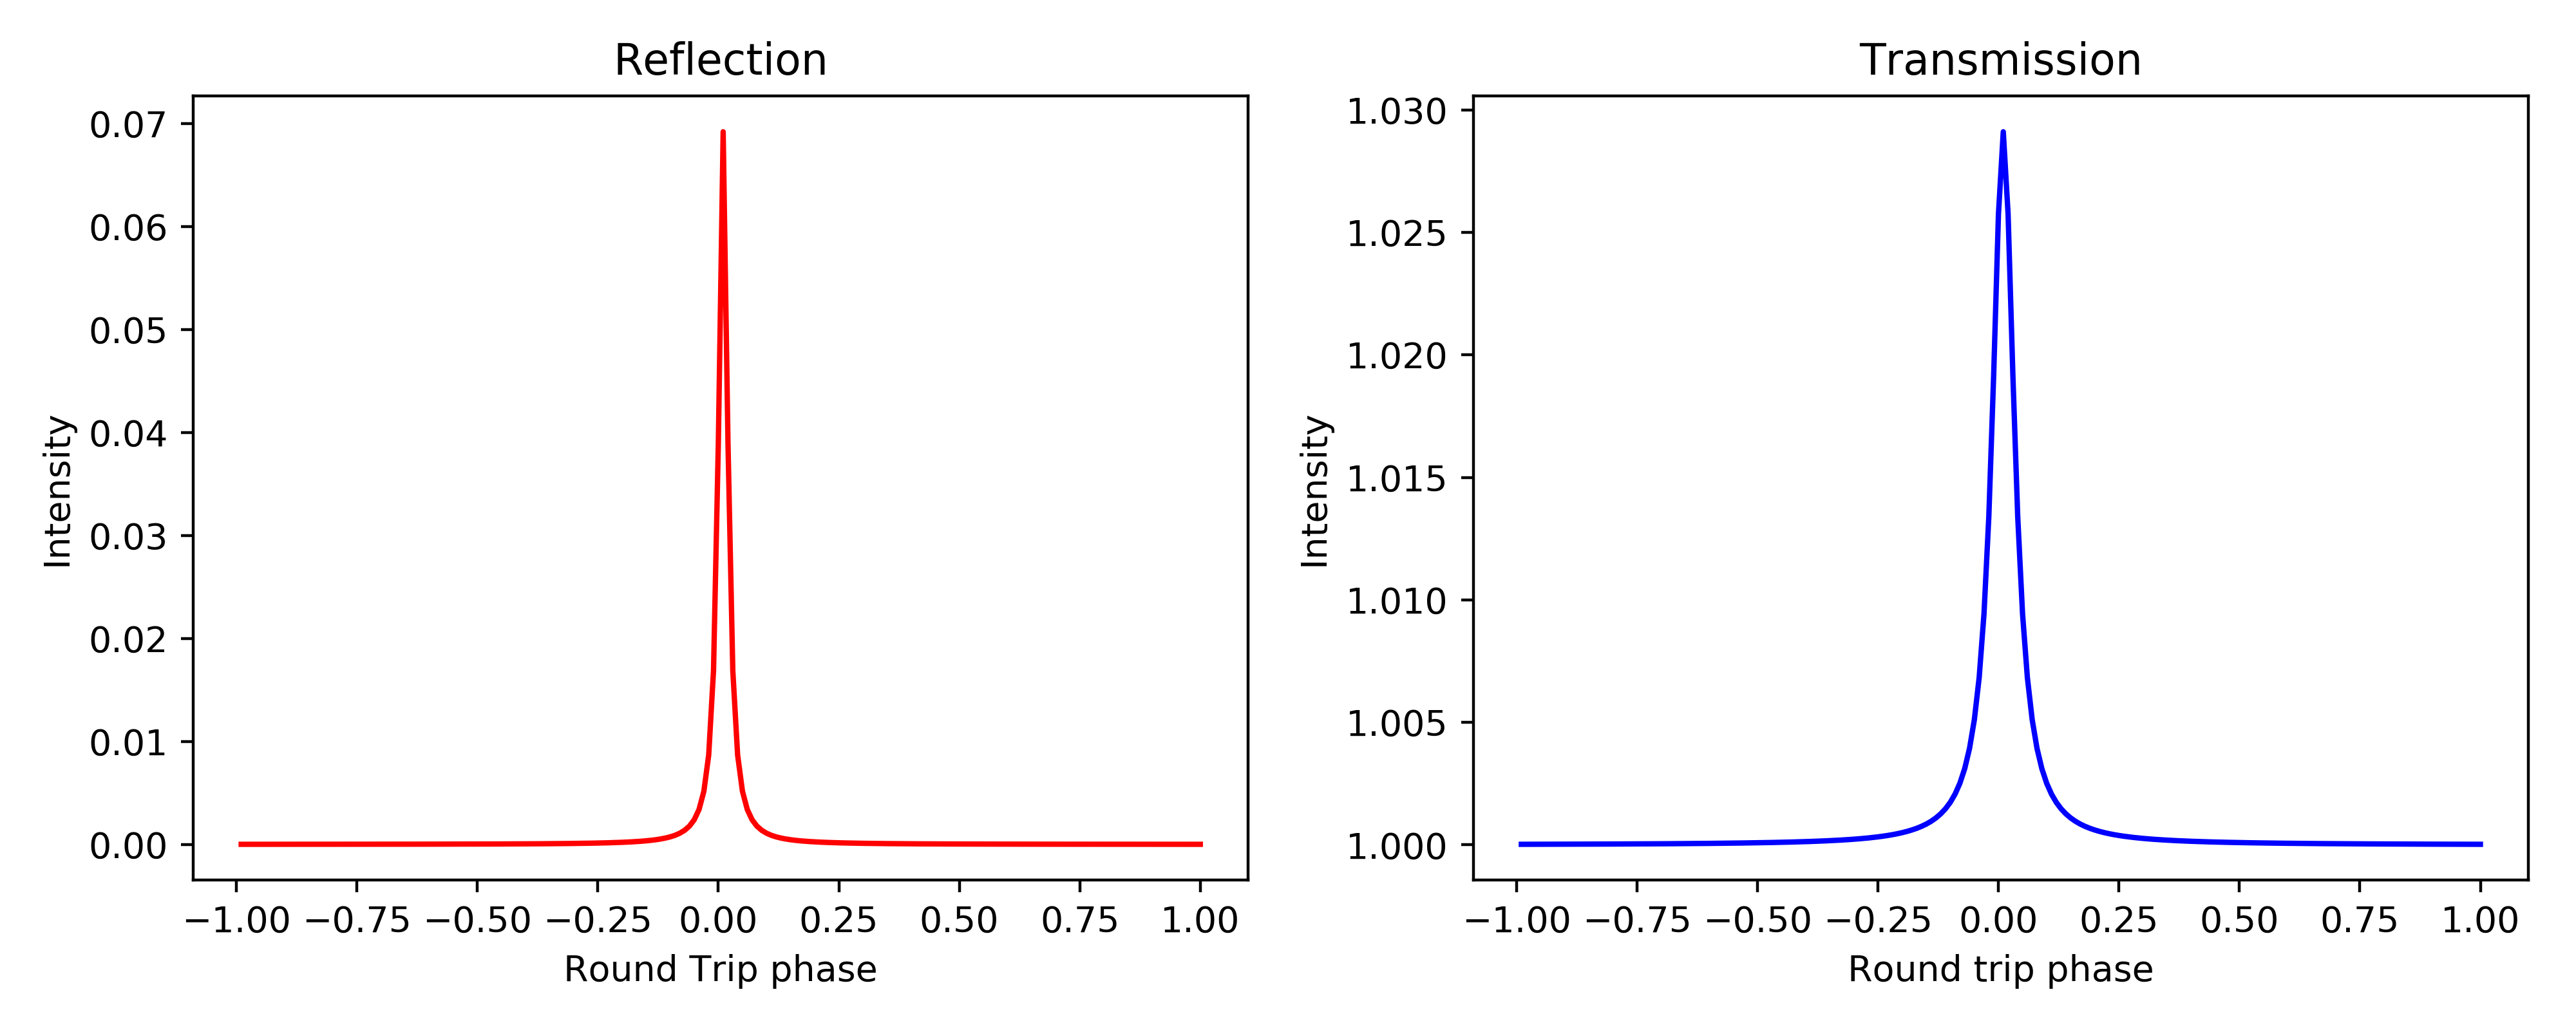
\includegraphics[width=0.85\textwidth]{add_drop_gain_plots.png}
\caption{Gain introduced into an all-pass resonator: we see clear difference in the intensities.}
\end{figure}

\subsection{Phasor Plots}
Now let us see how complex plots of Add drop is different from the All-pass resonator. Fig. 2.18 shows that the loop goes towards the negative real axis as the phase is increased. This tells a lot about the distinct behavior.

\begin{figure}[h]
\centering
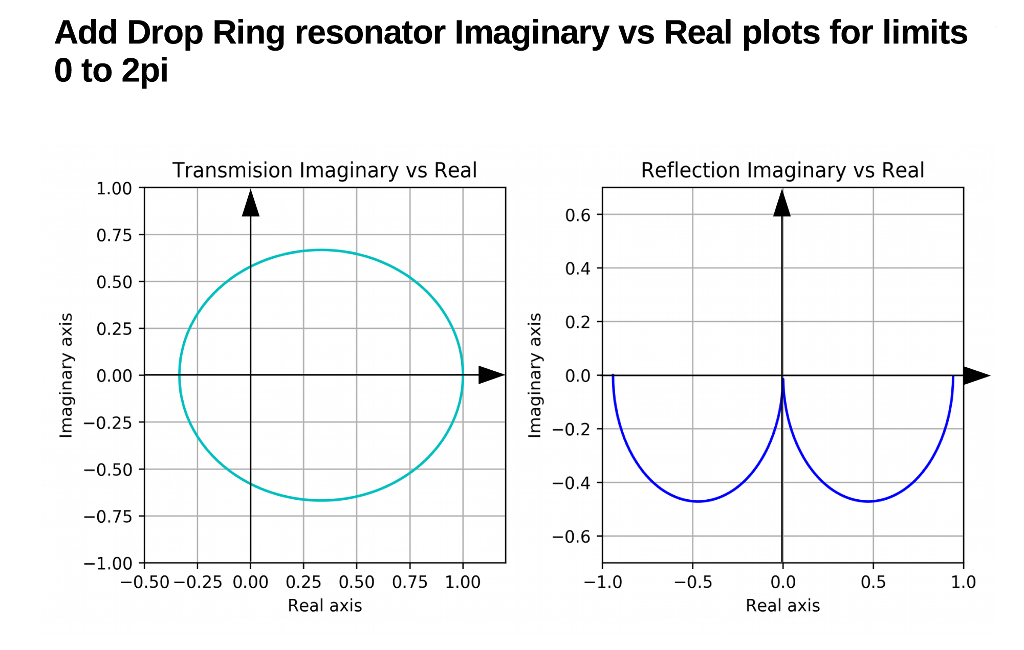
\includegraphics[width=1\textwidth]{ImagVsReal(add-drop).png}
\caption{Phaser plots of complex Transmitivity and Reflectivity of an add-drop ring resonator from 0 to $2\pi$}
\end{figure}


\section{Two Coupled Ring Resonator}
Now we turn another optical waveguide into a ring shape and install it on the top of the all-pass ring resonator such that now we have dual ring geometry and a waveguide coupler. This geometry does allow resonant behaviors and the spectra vary largely from an all-pass resonator.
In this arrangement, the coupling between the two resonators (rings) also plays an important role in the spectra of the light that passes through the resonator. Fig. 2.19 displays the basic geometry of the couple ring system we are going to discuss along with their energies. The circumference of these resonators are same for both rings given by $b = 25\mu m$, and the refractive index for these resonators is $n=3.45$ and the Quality Factors are given as $Q_{1} = 1\times10^{5}$ and $Q_{2} = 1\times10^{6}$

\begin{figure}[h]
\centering
\includegraphics[width=0.65\textwidth]{couple_ring_resonator.eps}
\caption{Illustrated fields and geometry of a coupled ring resonator}
\end{figure}

In this geometry, we will study the transmittance of the system as the symmetric case is its reflection in every case. The equation for complex transmitivity of this two resonator system is,

\begin{equation}
\frac{E_{t}}{E_{i}} = \frac{r_{1} - r_{12} a_{1} e^{i\phi_{1}}}{1 - r_{1} r_{12} a_{1} e^{i\phi_{1}}}
\end{equation}

where $r_{12}$ is the coupling parameter of the second resonator and is also a complex number given by,

\begin{align*}
r_{12} = \frac{r_{2} - a_{2} e^{i\phi_{2}}}{1 - r_{2} a_{2} e^{i\phi_{2}}}
\end{align*}


\subsection{Coupled Resonator Induced Transparency and Absorption}
Coupled resonator systems, like the one above, have been observed to display the quantum interference effects like Electromagnetically Induced Transparency and Electromagnetically Induced Absorption (EIT and EIA) via their optical analog known as Coupled Resonator Induced Transparency and Absorption (CRIT and CRIA) [3,4]. These quantum interference effects are observed in atoms with at least 3 energy levels but the similar optical analogs of these effects can be seen in these classical resonator systems. This enables enhanced dispersion and transitions from superluminal and subluminal group velocities at room temperature and in micro level scale. These effects will be discussed in detail using ring geometry optical microresonators in later chapters.

\newpage
\section*{References}
\addcontentsline{toc}{section}{References}
\paragraph{\normalfont \large $[1]$ J. Heebner, R. Grover, T. Ibrahim “Optical Microresonators, Theory, Fabrication, and Applications", Springer Science+Business Media (2008)\\
\\ $[2]$ K. Totsuka and M. Tomita “Dynamics of fast and slow pulse propagation through a microsphere–optical-fiber system", Phy. Rev. E \textbf{75} (2007)\\
\\ $[3]$ D. D. Smith, H. Chang, K. A. Fuller, A. T. Rosenberger, and R. W. Boyd, “Coupled-resonator-induced
transparency,” Phys. Rev. A \textbf{69}, 063804 (2004)\\
\\ $[4]$ A. Naweed, G. Farca, S. Shopova, and A. T. Rosenberger, “Induced transparency and absorption in coupled
whispering-gallery microresonators,” Phys. Rev. A \textbf{71} (2005).\\
\\ $[5]$ C. G. B. Garrett, and D. E. McCumber, “Propagation of a Gaussian light pulse through an anomalous dispersion medium." Phys. Rev. A \textbf{1}, 305 (1970).\\
\\ $[6]$ Chu, S. and Wong, S. “Linear pulse propagation in an absorbing medium.“ Phys. Rev. Lett. \textbf{48}, 738
(1982).\\
\\ $[7]$ R. Y. Chiao, Superluminal (but causal) propagation of wave packets in transparent media with inverted atomic populations. Phys. Rev. A \textbf{48}, R34 (1993).\\
\\ $[8]$ E. Bolda, J. C. Garrison, and R. Y. Chiao, “Optical pulse propagation at negative group velocities due to a nearby gain line." Phys. Rev. A \textbf{49}, 2938 (1994).\\
\\ $[9]$ R.W. Boyd and D. Gauthier “Controlling the Velocity of Light Pulses", Science \textbf{326} (2009)\\
\\ $[10]$ L. J. Wang, A. Kuzmich and A. Dogariu “Gain-assisted superluminal light propagation", Nature \textbf{406} (2000)\\
\\ $[11]$ K. J. Vahala, “Optical microcavities,” Nature \textbf{424}, 839 (2003).\\
\\ $[12]$ Z. Shi, R. W. Boyd, D. J. Gauthier, C. C. Dudley, “Enhancing the spectral sensitivity of interferometers
using slow-light media” Opt. Let. \textbf{32}, 8 (2007).\\
\\ $[13]$  M. Salit, G. S. Pati, K. Salit and M. S. Shahriar “Fast-light for astrophysics: super-sensitive gyroscopes and gravitational wave detectors” Journal of Modern Optics \textbf{54}, 16 (2007).\\
\\ $[14]$\,  Hecht, Jeff. The Laser Guidebook: Second Edition. McGraw-Hill, 1992. (Chapter 18-21).\\
\\ $[15]$  F. J. Duarte and L. W. Hillman (Eds.), Dye Laser Principles (Academic, New York, 1990).\\
\\ $[16]$ A. Naweed, “Photonic coherence effects from dual-waveguide coupled pair of co-resonant microring resonators", Opt. Exp. \textbf{23} (2015).\\
\\ $[17]$ L. V. Hau, S. E. Harris, Z. Dutton, and C. H. Behroozi, “Light speed reduction to 17 meters per second in
an ultracold atomic gas." Nature \textbf{397}, 594 (1999).\\
\\ $[18]$ M. M. Kash, et al. “Ultraslow group velocity and enhanced nonlinear optical effects in a coherently
driven hot atomic gas." Phys. Rev. Lett. \textbf{82}, 5229 (1999).\\
\\ $[19]$ D. Budker, D. F. Kimball, S. M. Rochester, and V. V. Yashchuk, “Nonlinear magneto-optics and reduced group velocity of light in atomic vapor with slow ground state relaxation." Phys. Rev. Lett. \textbf{83}, 1767 (1999).
\\ $[20]$ A. Einstein, H. A. Lorentz, H. Minkowski, H. and Weyl, “The Principle of Relativity, Collected Papers"
(Dover, New York, 1952).}